\section{The positivity conjecture}\label{sec:positivity}

\subsection{The statement and its hypothesis}\label{ssec:positivitystatement}

A single-centred supersymmetric black hole in four dimensions has a spherically symmetric horizon and carries no angular momentum. The helicity trace index $B_6$ of a quarter-BPS state is $-\frac{1}{6!}\Tr\big[(-1)^{2h}(2h)^6\big]$, and for a configuration whose only degrees of freedom beyond the horizon are the twelve fermion zero modes of the broken supersymmetries, the trace evaluates to $-1$ times the number of horizon states; the sign is fixed and the index is negative, that is, $d = -B_6 > 0$. Sen \cite{Sen11positivity} turned this into a conjecture about Fourier coefficients. In the region $\mathcal R$ of the axion--dilaton moduli space in which the attractor point of the charges $(Q,P)$ lies, bounded by walls of marginal stability, the single-centred black hole is the only configuration, and the Fourier coefficient \eqref{eq:dvv} taken with the contour of that region should be positive. For the heterotic string on $T^6$ the region is cut out by
\begin{equation}\label{eq:senconditions}
\begin{gathered}
Q\cdot P\ge 0,\qquad Q\cdot P\le Q^2,\qquad Q\cdot P\le P^2,\\
Q^2>0,\qquad P^2>0,\qquad Q^2P^2-(Q\cdot P)^2>0,
\end{gathered}
\end{equation}
(equation (3.7) of \cite{Sen11positivity}), and for the $\ZZ_2$ CHL model, whose duality group is $\Gamma_1(2)$, by
\begin{equation}\label{eq:z2conditions}
\begin{gathered}
Q^2>0,\qquad P^2>0,\qquad Q^2P^2>(Q\cdot P)^2,\\
2Q^2+P^2\ge 3(Q\cdot P)^2,\qquad 2Q^2\ge Q\cdot P,\\
P^2\ge Q\cdot P,\qquad Q\cdot P\ge 0
\end{gathered}
\end{equation}
(equation (3.9) there, with $Q^2$ normalised so that $NQ^2/2\in\ZZ$). Sen verified the positivity of $d(Q,P)$ on these cones for the heterotic string and for the CHL models $N=2,3,5,7$ in the range of charges of his Tables~1 to~5, and stated the conjecture for all charges in the cone. We have reproduced his Tables~1 and~2 exactly (Appendix~\ref{app:computation}).

The hypothesis of the argument is explicit in \cite{Sen11positivity}: the conclusion requires ``some duality frame in which only single centered black hole solution, whose only hair are the fermion zero modes associated with broken supersymmetry, contributes'' to the index. In the heterotic frame the quarter-BPS black hole does have hair beyond the fermion zero modes (the hair modes identified in \cite{BMS09hair}), but there is a frame, the type IIB frame on $K3\times T^2$, in which the hair reduces to the fermion zero modes; this is what makes the conjecture consistent there, and what was proved later.

\begin{theorem}[Bringmann--Murthy 2013]\label{thm:bringmannmurthy}
For type II string theory on $K3\times T^2$ (equivalently the heterotic string on $T^6$, the form $1/\Phi_{10}$) and on $T^6$ (the $\mathcal N=8$ theory), the single-centred indices in the attractor region are positive for the classes of charges treated in \cite{BringmannMurthy13}; the proof uses the mock modular decomposition of the Fourier--Jacobi coefficients of $1/\Phi_{10}$ \cite{DMZ12}.
\end{theorem}

The restriction to classes of charges was removed by Rossell\'o \cite{Rossello24}, who bounds the tail of the Rademacher expansion of the mock Jacobi forms $\psi^F_m$ of \cite{DMZ12} against its leading term.

\begin{theorem}[Rossell\'o 2024]\label{thm:rossello}
For type II string theory on $K3\times T^2$, the single-centred index $d^*(m,n,\ell)$, with $m = P^2/2$, $n = Q^2/2$, $\ell = Q\cdot P$, is positive for every $m,n\ge 1$ with $4mn-\ell^2>0$: for $n\ge m$ and $0\le \ell\le m$ one has $(-1)^{\ell+1}c^F_m(n,\ell)>0$, and the general case follows by the $S$-duality invariance of the single-centred index.
\end{theorem}

\begin{verdict}[claim 9, heterotic and CHL]
Proved for the heterotic string on $T^6$, by Theorems~\ref{thm:bringmannmurthy} and~\ref{thm:rossello}; our scan of the single-centred cone up to $Q^2\le 12$, $P^2\le 6$, $Q\cdot P\le 4$ (Appendix~\ref{app:computation}) agrees. For the CHL orbifolds no counterexample is known, our scan for $N=2$ finds only positive indices, and no proof exists: the Rademacher bound of \cite{Rossello24} has not been carried out for the mock Jacobi forms of $1/\Phit_k$, and \cite{Rossello24} names this as the next case. The conjecture is proved in the model in which it was first stated and confirmed in the CHL models.
\end{verdict}

\subsection{The failure in the toroidal orbifolds}\label{ssec:toroidal}

Sen's paper states the conjecture as a consequence of the black hole argument for ``the $\mathcal N=4$ supersymmetric string theories'', and the subsequent literature \cite{CD19,CKMRW20} tested it in the full list of $\mathcal N=4$ compactifications with known dyon partition functions. Chattopadhyaya and David \cite{CD19} found that it fails in two of them: the freely acting $\ZZ_2$ and $\ZZ_3$ orbifolds of type IIB on $T^6$, in which the orbifold acts by a reflection of four coordinates of $T^4$ (or a rotation by $2\pi/3$ of two planes) together with a shift of half (or a third) of a circle of the remaining $T^2$. The $\ZZ_2$ model has the twisted elliptic genera
\begin{equation}\label{eq:tor2genera}
\begin{aligned}
F^{(0,0)} &= 0,& F^{(0,1)} &= \tfrac83 A - \tfrac43 B\,E_2(\tau),\\
F^{(1,0)} &= \tfrac83 A + \tfrac23 B\,E_2(\tfrac\tau2),& F^{(1,1)} &= \tfrac83 A + \tfrac23 B\,E_2(\tfrac{\tau+1}2),
\end{aligned}
\end{equation}
where $A = \sum_{i=2}^4\theta_i(\tau,z)^2/\theta_i(\tau,0)^2$, $B = \theta_1(\tau,z)^2/\eta(\tau)^6$, and $E_2(\tau) := 2E(2\tau) - E(\tau)$ is the weight-two form of $\Gamma_0(2)$ built from the Eisenstein series $E(\tau) = 1 - 24\sum\sigma_1(n)q^n$ (this is the $E_N$ of \cite{DJS06}; it is not the quasi-modular Eisenstein series, and the two are easily confused). The Siegel form is $\Phit_2 = \Phit_6^2/\Phit_{10}$, of weight two, with the prefactor $e^{2\pi i(\rho+v)}$ in place of $e^{2\pi i(\rho+\sigma/N+v)}$ in \eqref{eq:product}, and the index is given by \eqref{eq:dvv} with $Q^2\in\ZZ$, $P^2\in 2\ZZ$. The single-centred region is again cut out by \eqref{eq:z2conditions}, since the duality group is again $\Gamma_1(2)$.

\begin{theorem}[claim 9 fails as stated]\label{thm:positivityfails}
In the $\ZZ_2$ toroidal orbifold of type IIB on $T^6$, the index $d(Q,P)$ computed from \eqref{eq:dvv} with the contour of the attractor region is negative for infinitely many charges satisfying the single-centred conditions \eqref{eq:z2conditions}. In the range $Q^2\le 12$, $P^2\le 8$, $Q\cdot P\le 4$ there are exactly twenty-one such charges, listed in Table~\ref{tab:violations}; the first ones are
\begin{gather*}
d(1,2,0) = -224,\quad d(1,4,0) = -1248,\\
d(2,2,1) = -256,\quad d(3,2,0) = -3392,\\
d(3,4,0) = -10320,
\end{gather*}
in the notation $d(Q^2,P^2,Q\cdot P)$. In the first column of Table~\ref{tab:tor2} ($P^2=0$, outside the cone) the sign is $(-1)^{Q^2}$ for $Q^2\le 12$; Figure~\ref{fig:indices} draws the table.
\end{theorem}

\begin{figure}[t]
\centering
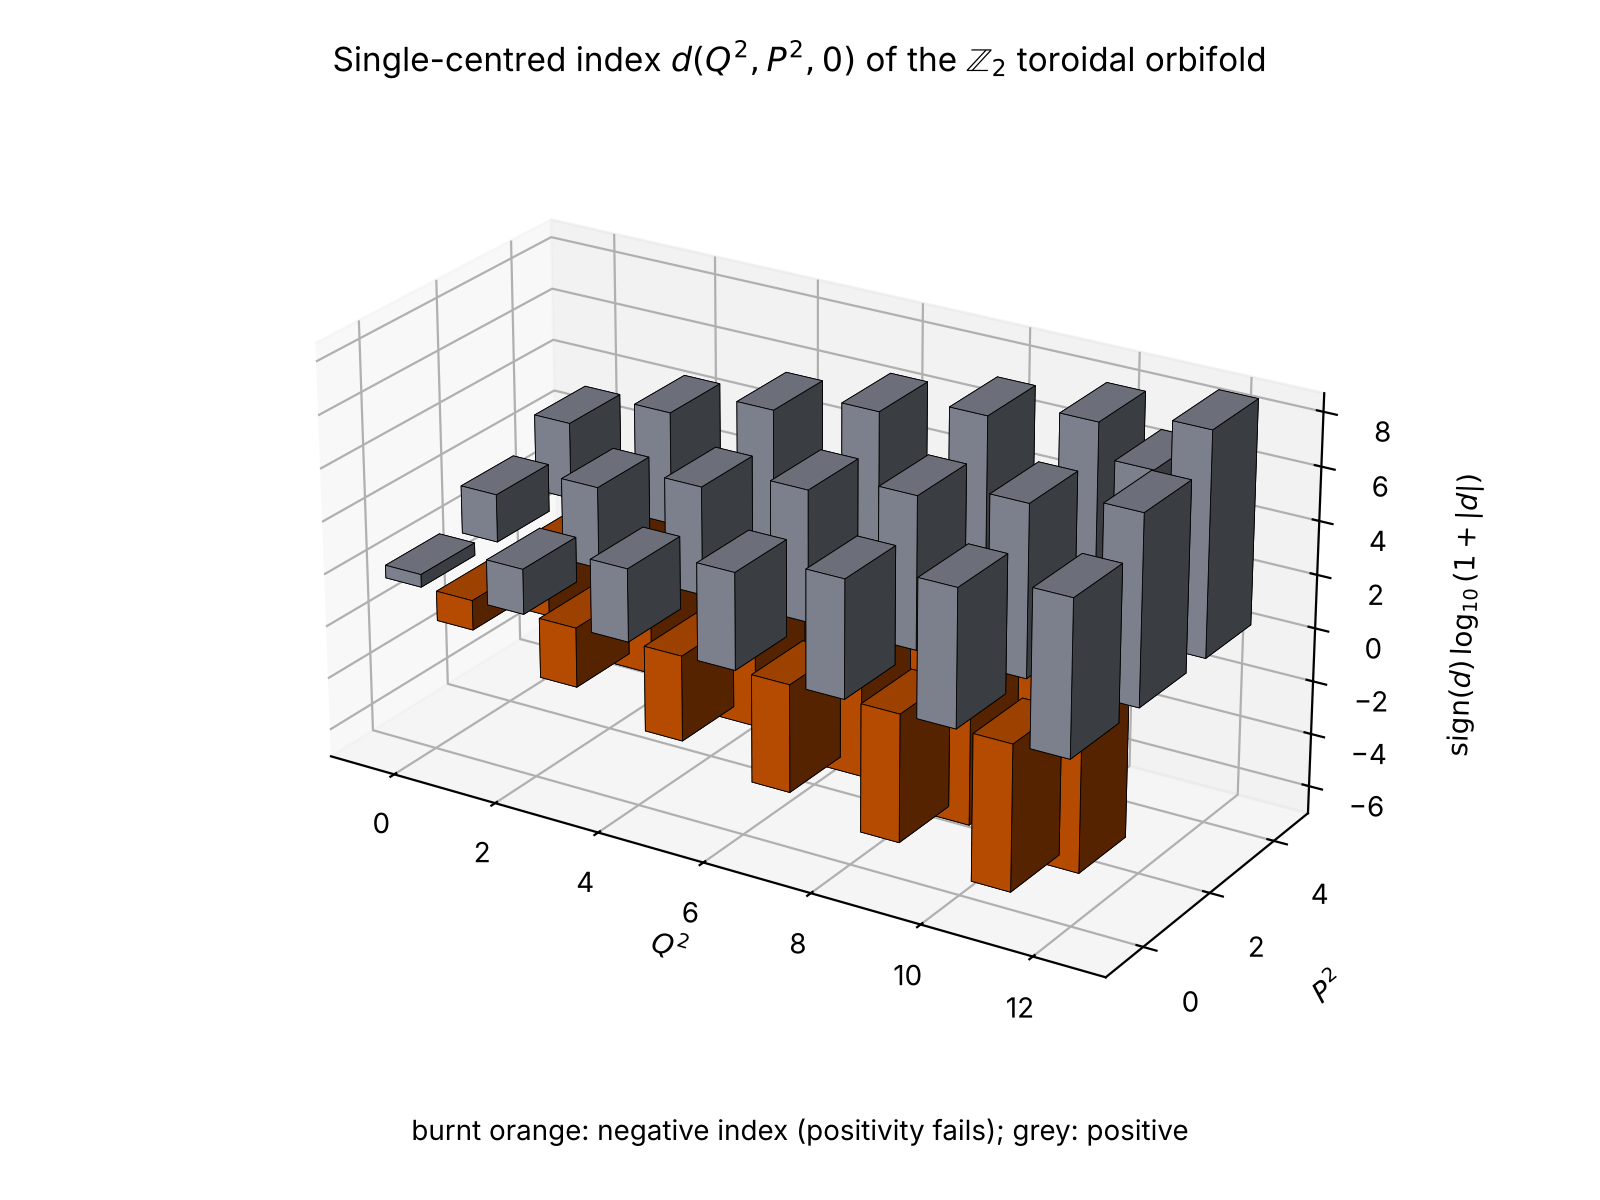
\includegraphics[width=\columnwidth]{figures/fig_indices.png}
\caption{The single-centred index $d(Q^2,P^2,0)$ of the $\ZZ_2$ toroidal orbifold from Table~\ref{tab:tor2}, drawn on the scale $\mathrm{sign}(d)\log_{10}(1+|d|)$. Every bar in burnt orange is a negative index; along $P^2 = 2$ the sign alternates with $Q^2$, and every odd $Q^2$ lies inside the cone \eqref{eq:z2conditions} of Theorem~\ref{thm:positivityfails}.}
\label{fig:indices}
\end{figure}

\begin{proof}
We expanded the product \eqref{eq:product} for the genera \eqref{eq:tor2genera} in exact rational arithmetic, with the Fourier coefficients of the theta functions, of $\eta^{-6}$ and of the Eisenstein series computed from their definitions, and read off the coefficients of $e^{2\pi i(Q^2\rho + (P^2/2)\sigma/2 + Q\cdot P\,v)}$ in the expansion in which the factor $(1-e^{-2\pi i v})^{-2}$ at $k'=l=0$ is expanded in powers of $e^{-2\pi iv}$ (the attractor region for $Q\cdot P\ge 0$). The resulting tables agree entry by entry with Tables~17, 18 and~19 of \cite{CD19} in their common range. The twenty-one charges of Table~\ref{tab:violations} satisfy each inequality of \eqref{eq:z2conditions} by inspection and have negative index. For the infinitude: the values at $P^2=2$, $Q\cdot P=0$ are
\[
\begin{gathered}
64,\ -224,\ 1152,\ -3392,\ 11520,\ -30336,\ 83968,\\
-202560,\ 496512,\ -1118496,\ 2521600,\ -5374656
\end{gathered}
\]
for $Q^2 = 0,1,2,\dots,11$; every odd $Q^2$ with $P^2 = 2$, $Q\cdot P = 0$ lies in the cone \eqref{eq:z2conditions}, and \cite[Section~4.1]{CD19} show from the Fourier--Jacobi coefficient $\psi_1$ of $1/\Phit_2$ at $P^2=2$ that the finite part of $\psi_1$, which is what the single-centred index is, has coefficients of alternating sign in $Q^2$; the alternation is visible in our table for $Q^2\le 12$. The analogous statement for the $\ZZ_3$ orbifold is \cite[Section~4.2]{CD19}.
\end{proof}

\begin{table}[t]
\centering
\footnotesize
\begin{tabular}{@{}rrrr@{\qquad}rrrr@{}}
\toprule
$Q^2$ & $P^2$ & $Q\cdot P$ & $d$ & $Q^2$ & $P^2$ & $Q\cdot P$ & $d$ \\
\midrule
1 & 2 & 0 & $-224$   & 7 & 2 & 0 & $-202560$ \\
1 & 4 & 0 & $-1248$  & 7 & 2 & 2 & $-30336$ \\
2 & 2 & 1 & $-256$   & 7 & 4 & 0 & $-179022$ \\
3 & 2 & 0 & $-3392$  & 8 & 2 & 1 & $-220672$ \\
3 & 4 & 0 & $-10320$ & 9 & 2 & 0 & $-1118496$ \\
4 & 2 & 1 & $-3840$  & 9 & 2 & 2 & $-202560$ \\
5 & 2 & 0 & $-30336$ & 9 & 4 & 0 & $-155232$ \\
5 & 2 & 2 & $-3392$  & 10 & 2 & 1 & $-1204992$ \\
5 & 4 & 0 & $-55424$ & 11 & 2 & 0 & $-5374656$ \\
6 & 2 & 1 & $-33536$ & 11 & 2 & 2 & $-1118496$ \\
  &   &   &          & 12 & 2 & 1 & $-5741824$ \\
\bottomrule
\end{tabular}
\caption{The twenty-one charges with $Q^2\le 12$, $P^2\le 8$, $Q\cdot P\le 4$ in the single-centred cone \eqref{eq:z2conditions} of the $\ZZ_2$ toroidal orbifold whose index is negative. The entries $d(Q^2,2,0)$ for odd $Q^2$ and $d(Q^2,2,2) = d(Q^2-2,2,0)$ continue indefinitely with alternating sign.}
\label{tab:violations}
\end{table}

\subsection{Which hypothesis fails}\label{ssec:hair}

The conjecture is a theorem of black hole physics applied to a Fourier coefficient under one hypothesis, the existence of a frame without hair. The $\ZZ_2$ and $\ZZ_3$ toroidal orbifolds are the only known $\mathcal N=4$ compactifications with $\sum_{r,s}F^{(r,s)} = 0$, that is, in which the untwisted elliptic genus $F^{(0,0)}$ vanishes because the orbifold acts on $T^4$ rather than on K3. Chattopadhyaya and David \cite{CD21} then carried out the programme of \cite{BMS09hair}: in the type IIB frame they identified the hair modes of the quarter-BPS dyon in every CHL model and in the two toroidal orbifolds, removed their contribution from the index, and found that the index of the remaining horizon states is positive in every case, including the toroidal orbifolds. The combination of the two results is the precise statement of what fails.

\begin{proposition}[the hypothesis]\label{prop:hypothesis}
In the $\ZZ_2$ and $\ZZ_3$ toroidal orbifolds of type IIB on $T^6$ there is no duality frame in which the single-centred quarter-BPS dyon has no hair beyond the fermion zero modes of broken supersymmetry. The index of the horizon states, obtained by removing the hair in the type IIB frame, is positive on the single-centred cone in the range tested in \cite{CD21}.
\end{proposition}

\begin{proof}
If such a frame existed, the argument of \cite{Sen11positivity} would apply in it and the index would be positive on the cone, contradicting Theorem~\ref{thm:positivityfails}; the index is frame independent. The second statement is the computation of \cite{CD21}, Sections~4 and~5.
\end{proof}

\begin{verdict}[claim 9, all $\mathcal N=4$ models]
False as stated. The sentence of \cite{Sen11positivity} that leads to the conjecture, \fatal{that the index of single-centred black holes is positive in $\mathcal N=4$ string theories}, holds in the heterotic string and the CHL models and fails in the two toroidal orbifolds, where the quarter-BPS black hole carries hair in every frame. The corrected statement is the one proved in \cite{CD21} and stated in Proposition~\ref{prop:hypothesis}: the index of the horizon states, after the hair is removed, is positive. Sen's paper does not claim the toroidal orbifolds, which it does not mention, and it states the hypothesis under which its argument works; the failure is of the general sentence, not of the argument. We record it as a failure because the general sentence is what the paper's title and abstract assert, and because the literature took it as a conjecture about all $\mathcal N=4$ compactifications \cite{CD19,CKMRW20}.
\end{verdict}

\begin{verdict}[claim 10]
Confirmed. The hair modes of the quarter-BPS black hole were identified in the type IIB frame for $K3\times T^2$ in \cite{BMS09hair} and for every CHL model and both toroidal orbifolds in \cite{CD21}, and in each case the remaining horizon index is positive. The identification rests on the classification of the supersymmetric deformations of the black hole solution that are supported outside the horizon, which is complete for the fields of the two-derivative supergravity and has not been extended to the full string spectrum; this is the missing step, and no paper has supplied it.
\end{verdict}

\begin{verdict}[claim 36]
Confirmed. The companion of the positivity conjecture is the statement of \cite{CGMS16} that every microstate of a single-centred BPS black hole, once the fermion zero modes of broken supersymmetry are removed, carries zero angular momentum, so that the index counts the states with sign $+1$ and positivity follows. It was tested in \cite{CGMS16} on the quarter-BPS states of type IIB on $T^6$ at low charges by an explicit enumeration of the supersymmetric configurations of D-branes, and in \cite{HeidmannMondal19} on multi-centred configurations with pure D-brane charges, and holds in every case computed. It is not proved, and the toroidal orbifolds show what its proof must contain: there the index of the full dyon is negative, so either some microstates carry angular momentum or the hair modes do, and \cite{CD21} locates the sign in the hair. Later tests at higher charges \cite{ChowdhuryMaji24,ChowdhuryMaji26} reproduce the index of the pure D-brane system by algebraic geometry and find no state of nonzero angular momentum. Positivity of the index, now a theorem for $K3\times T^2$ (Theorem~\ref{thm:rossello}), does not imply the statement, as \cite{Rossello24} notes: an index that is positive can still count fermionic states. We have searched the thirty-two papers citing \cite{CGMS16} and found no proof; the statement for the horizon states remains open and consistent with every test.
\end{verdict}

\begin{remark}\label{rem:normalisation}
The numbers of Theorem~\ref{thm:positivityfails} are the index $d = -B_6$ with the sign $(-1)^{Q\cdot P+1}$ included and without the factor $1/N$ written in front of the contour integral in \cite{CD19}: the integral over $\sigma$ runs over a period of length $N$ and produces a factor $N$ that cancels it. The same normalisation reproduces Sen's Table~2 for the CHL model, which fixes it.
\end{remark}
